\documentclass[
 a4paper,twocolumn,showpacs,aip,groupedaddress,%
  eqsecnum,notitlepage,showkeys,cha,longbibliography,10pt
]{revtex4-1}
\usepackage[english]{babel}
\usepackage[utf8x]{inputenc}
\usepackage[T1]{fontenc}
\usepackage{amssymb}
\usepackage{amsmath,latexsym}
\usepackage{subcaption}
\usepackage{graphicx}
\usepackage{dcolumn}
\usepackage{tikz}
\usepackage{natbib}
\usepackage{float}
\usepackage[export]{adjustbox}
\usepackage{hyperref}
\usepackage{mathtools}
\usepackage{soul}
\DeclarePairedDelimiter\bra{\langle}{\rvert}
\DeclarePairedDelimiter\ket{\lvert}{\rangle}
\DeclarePairedDelimiterX\braket[2]{\langle}{\rangle}{#1 \delimsize\vert #2}

\newcommand*{\citen}[1]{%
  \begingroup
    \romannumeral-`\x % remove space at the beginning of \setcitestyle
    \setcitestyle{numbers}%
    \cite{#1}%
  \endgroup   
}

\usepackage[a4paper,top=1.8cm,bottom=1.8cm,left=1.5cm,right=1.5cm]{geometry}
\usepackage[skip=5pt, font=scriptsize, labelfont=bf, justification=raggedright]{caption}

\usepackage{titlesec}

\titlespacing\section{0pt}{12pt plus 4pt minus 2pt}{0pt plus 2pt minus 2pt}

\graphicspath{ {Images/} }

\begin{document}

\title{\Large{Atomic Magnetometer Developments for Medical Applications}}

\author{Lindsey Keary}
\affiliation{ 
Student Number : 17099595, l.keary.17@ucl.ac.uk, University College London
}
\date{\today}

\maketitle
\section{Introduction}
Magnetic field sensing has a vast variation in applications across a number of fields including: navigation, geophysics, archeology and diagnostic medicine \citep{Budker2007OpticalMagnetometry,Khedr2017AApplications}. Biomagnetic sensing is an active area of research where the development of diagnostic techniques such as: magnetoencephalography (MEG), magnetocardiography (MCG), magnetic resonance imaging (MRI) and magnetic induction sensing (MIT) aid in diagnosing and treating many medical conditions. MEG provides a noninvasive method to detect brain activity through detection of the very weak < 1 pT magnetic field response. Commercial MEG systems currently consist of $\approx$ 200 superconducting quantum interference devices (SQUIDs) in an array \citep{Sander2012MagnetoencephalographyMagnetometer.}. However, it is extremely expensive to build and operate these MEG systems due to the requirement for cryogenic cooling \citep{Knappe2014Optically-PumpedMEG}. It is critical that a more affordable alternative option is developed such that continuous measurements of brain responses expands our understanding of typical and atypical brain operation. Therefore, more accessible MEG systems would enable clinical trails and research into treatment of patients with mental health illness such as schizophrenia, dementia, depression, and epilepsy \citep{Johnson2010MagnetoencephalographyMagnetometer}.

NIST is a leader in pioneering chip-scale sensing device development. The first atomic clock developed in 2004 used microelectro-mechanical systems (MEMS) technology could also be operated as an atomic magnetometer (AM). The sensitivity of 40 fTHz$^{-1/2}$ was achieved using coherent population trapping as the pumping technique \citep{Schwindt2004Chip-scaleMagnetometer}. Improved operation schemes and development of the spin-exchange relaxation (SERF) regime enables measurement of biomedical fields with a significant increase in sensitivity \citep{Allred2002High-SensitivityRelaxation}. AM development is currently under investigation as a replacement for SQUID MEG systems. The AM operational sensitivity is approaching the 3–4 fTHz$^{-1/2}$ sensitivity of commercial SQUID MEG systems \citep{Shah2013AApplications}. The key advantage of employing AM arrays is that they do not require cryogenic cooling. Consequently fabrication is more cost-efficient and the sensors can be placed closer to the target \citep{Boto2017AMagnetometers}.  Additionally, AMs also show potential for diagnosing atrial fibrillation by completing MIT \citep{Deans2016OpticalHeart}.  


\section{\label{sec:level1}Atomic Magnetometers}
Atomic, or as they are also often referred to as optical, magnetometers are devices which determine the local magnetic field by measuring the Larmor precession by optically probing a specific atomic transition \citep{Kitching2008MicrofabricatedApplications}. Larmor precession occurs due to the magnetic moment of particles, such as electrons and atomic nuclei, experiencing a torque when a magnetic field is applied. The Larmor frequency is given by: 

\begin{equation}
\label{eq:interactionham0}
\omega_{L}=\gamma B,
\end{equation}
%The interaction Hamiltonian is $H_{int}=\vec{\mu}\cdot\vec{B}$ for either particle.
where the gyromagnetic constant, $\gamma$, is the ratio of the magnetic moment, $\vec{\mu}$ to the total angular moment, $\vec{J}$. The magnitude of the magnetic field is given by $B$ \citep{Kitching2011AtomicReview}. Since electrons are fermions, the magnetic moment occurs due to the $\frac{1}{2}$- spin properties of the particles. In addition the atomic nucleus has a smaller magnetic moment, $\vec{\mu}_I$, resulting from the nuclear spin, $\vec{I}$ \citep{Foot2005AtomicPhysics}. Since the valence electron and nucleus form a coupled system for alkali atoms, $B$ results in precession of the electron spin which also forces the nuclear spin to rotate in the same direction \citep{Seltzer2008AtomicMagnetometery}. 

\subsection{Alkali Atomic Structure}
\begin{figure}[b]
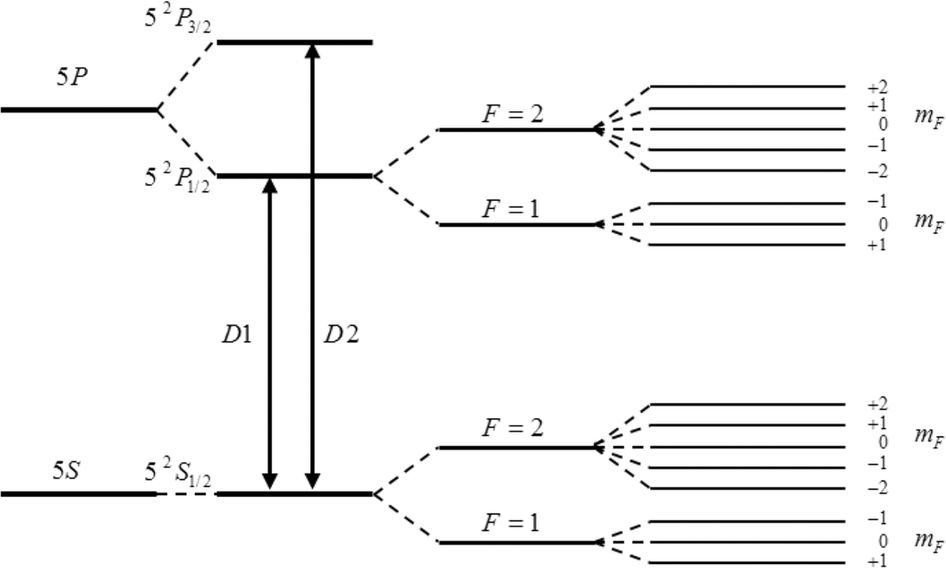
\includegraphics[height=0.25\textwidth,keepaspectratio,]{zeemspec}
\caption{\label{fig:zeemspec}Spectroscopic structure of alkali metal ($^{87}Rb$) atoms with $m_{F}$ degeneracy lifted. The hyperfine and Zeeman sublevels of the second excited state are omitted \citep{Li2017EllipticalVapor}.}
\end{figure}

It is useful to initially consider the atomic energy structure alkali atoms as shown in Fig. (\ref{fig:zeemspec}). The fine structure arises from relativistic effects of the electron spin-orbit interaction. For the same principle quantum number $n$, there is a shift in energy for different values of $J$ \citep{Steane2002AtomicMatter}. The total angular momentum of the valence electron is: 

\begin{equation}
\label{eq:interactionham0}
\vec{J}=\vec{L}+\vec{S}, 
\end{equation}


where $\vec{S}$ is the electron spin angular momentum and $\vec{L}$ is the orbital angular momentum. When the valence electron is in the ground state, $\vec{L} = 0$. When the electron is in the first excited state, $\vec{L}=1$. The spectroscopic notation used is $n^{2S+1}L_{J}$ for the fine structure where the $\vec{L} = 0, 1, ...$ is associated with the $'S','P',...$ shell letters. The energy transitions between the ground 'S' state and the excited 'P' states are known as $D$-line transitions as shown in Fig. (\ref{fig:zeemspec}) \citep{Foot2005AtomicPhysics,LandiDeglInnocenti2014AtomicProcesses}.  

The hyperfine energy splitting occurs due to the interaction between the spin of the atomic nucleus and the electron spin. The total atomic angular momentum is:

\begin{equation}
\label{eq:interactionham0}
\vec{F}=\vec{I}+\vec{J},
\end{equation}
\\
where $\vec{F}$ points parallel to $\vec{J}$. $\vec{I}$ is the sum of the proton and neutron $\frac{1}{2}$-spin particles for a specific isotope \citep{LandiDeglInnocenti2014AtomicProcesses}. The Zeeman effect occurs in the presence of a magnetic field and results in further energy splitting of $\Delta E_{L}=\hbar\omega_{L}$ into Zeeman sublevels $m_{F}=\{-F,-F+1 ... F-1,F\}$ \citep{Seltzer2008AtomicMagnetometery}. 

\subsection{Pumping and Probing} 

\begin{figure}[b]
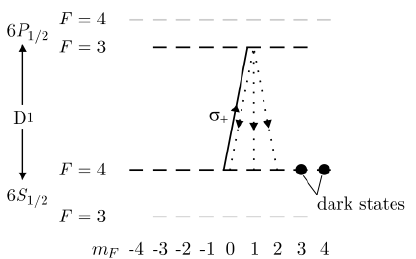
\includegraphics[height=0.3\textwidth,keepaspectratio,]{opticalpumping}
\caption{\label{fig:pumprobe} $\sigma_{+}$ beam pumping atoms into the Dark states \citep{Birzhandi2013EffectPhenomenon}.}
\end{figure}
 \begin{figure}[t]
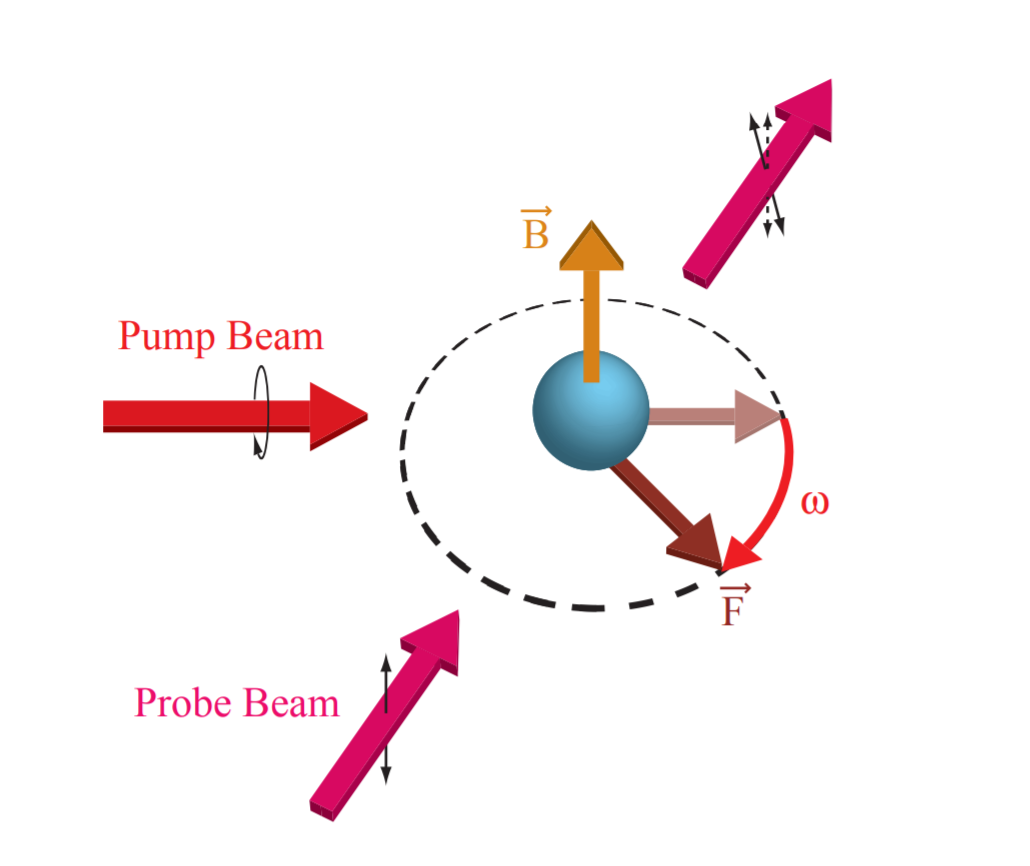
\includegraphics[height=0.3\textwidth,keepaspectratio,]{pumprobe}
\caption{\label{fig:opticalpumping} Schematic diagram of a pump-probe atomic magnetometer scheme. The circularly polarised pump beam produces a polarisation orientation of the atomic spins in the direction of laser propagation. In the presence of a weak magnetic field the angular momentum of the atom precesses at $\omega_{L}$ around $\vec{B}$. The output linearly polarised probe has undergone a plane rotation angle corresponding to the component of $\vec{S}$ in that direction \citep{Seltzer2008AtomicMagnetometery}.}
\end{figure}

The evolution of the valence electron spin of the alkali atoms can be used to detect weak $B$ fields. A circularly polarised beam is used align the valence electron spin, such that the atomic vapor becomes magnetised \citep{Sander2012MagnetoencephalographyMagnetometer.}. Circularly polarised light which is resonant with the D1 transition line pumps atoms into Dark states and produces a polarisation of the atomic spin parallel to the direction of propagation of the applied field \citep{Groeger2006AMagnetometer}. $\sigma^{+}$ polarised light excites atoms from a hyperfine ground state to the hyperfine exited $P_{\frac{1}{2}}$ state where $m_{F}$ is increased by +1  \citep{Birzhandi2013EffectPhenomenon}. The atomic selection rules \citep{Steane2002AtomicMatter} dictate that the atom can spontaneously decay to the $\ket{S_{\frac{1}{2}}, m_{F}=\{-1,0,1\}}$ states. If this transition is continually pumped the atoms will be transferred into Dark states which are optically transparent to the incoming laser photons. As shown in Fig. (\ref{fig:opticalpumping}) since there is no possible excited state transition.      

When all the atoms are transferred to Dark states the maximum transmission of photons through the cell is detected. The Larmor precession of the atomic spin around $\vec{B}$ results in a phase accumulation. Various detection methods have been implemented including detecting the modulation of the pump light transmission intensity and phase when a static $B_{0}$ field is applied at 45$^{\circ}$ to the pump beam and a radio frequency (rf) magnetic field $B_{1}(t)$ resonant with $\omega_{L}$ is applied perpendicular to $B_{0}$ \citep{Schwindt2007Chip-scaleTechnique,Groeger2006AMagnetometer}. Additionally, the output rotation angle of a linearly polarised probe laser is related to the degree of $\vec{S}$ in that direction  \citep{XiaMagnetoencephalographyMagnetometer,Kominis2003AMagnetometer}. The advantage of this scheme compared to the rf AM scheme is that the laser intensity noise is reduced and small angle polarisation rotations can be detected \citep{Budker2007OpticalMagnetometry}.  

The combination of homogeneous, natural and pressure, broadening of the transition linewidth and Doppler broadening of alkali metal atoms contained in a vapor cell results in a Voigt lineshape. At room temperature, the Doppler broadening linewidth is $\approx 0.5$ GHz for a alkali metal vapor cell \citep{Yariv2006PhotonicsCommunications,Siddons2008AbsoluteExperiment}. The ability to resolve transitions between hyperfine levels depends on the degree of Doppler broadening in comparison to the hyperfine $F \rightarrow F^{'}$ transition frequency. Transitions between a $F$ ground state and $F^{'}$ excited state can be driven using a dichroic atomic vapor laser lock (DAVLL) where the frequency stabilisation is $\approx 1$ MHz/h \citep{Bison2004DevelopmentCardio-magnetometer,Imanishi2005FrequencyCell}. 

\subsection{Sensitivity}
Initially the AM signal-to-noise ratio (S/N) was the limited by the $B$ field detection sensitivity. To increase the signal, the density of atoms in the vapor was increased \citep{Kitching2011AtomicReview}. However, as the atomic density was increased the number of collision events increased. The coherence time $T_{2}$ of the atomic spin is limited by atom collisions with the cell walls and atom-atom collisions. Complete depolarisation of the atomic spin occurs when alkali atoms collide with the cell walls or buffer gas atoms \citep{Budker2007OpticalMagnetometry}. The spin-exchange interaction occurs when alkali metal atoms have collisions with other alkali atoms. The spin-exchange interaction occurs rapidly such that the nuclear spin is unaffected. The total spin of the particles $\vec{S}=\vec{S}_{1}+\vec{S}_{2}$ is conserved but at least one spin value will change \citep{Happer1977EffectVapors}. The decoherence of the alkali spin influences the fundamental measurement sensitivity of an atomic magnetometer as: 

\begin{equation}
\label{eq:interactionham0}
\delta B =\frac{1}{\gamma\sqrt{N T_{2} t}},
\end{equation}

which is shot-noise limited \citep{Kominis2003AMagnetometer}. The measurement duration time and the number of alkali metal atoms are given as $t$ and $N$, respectively. 

\subsection{SERF magnetometer}
The development of the alkali-alkali spin-exchange relaxation-free (SERF) technique is demonstrated experimentally in Ref.[\citen{Allred2002High-SensitivityRelaxation}] to increase the magnetometer's sensitivity. The concept initially appears counterproductive to reducing transition broadening. Firstly the potassium atomic number density in the vapor cell to increased to $n = 10^{14}$ cm$^{3}$ thereby increasing the spin-relaxation rate to $T_{2}$ > 1/$\omega_{L}$. In this regime the two hyperfine ground states are described as being "locked" together and precesses slowly around a small, near zero, $B_{y}$ field in the direction of the highest occupation $F$ state. Transition broadening now is limited by collisions where $\vec{S}$ is not conserved, but the rate of these collisions is small comparatively. The theoretically achievable shot-noise limited sensitivity is $2 \times 10^{-18}$ THz$^{-1/2}$ and the measured sensitivity is 10 fTHz$^{-1/2}$ which is limited by current fluctuation noise from the magnetic shielding. The SERF technique can eliminate alkali-alkali spin-relaxation when measuring magnetic fields up to $\approx10$ nT \citep{Budker2007OpticalMagnetometry}. In Ref. [\citen{Kominis2003AMagnetometer}] using the SERF technique, the 0.54 fTHz$^{-1/2}$ sensitivity of the atomic magnetometer is demonstrated for a vapor cell of volume 0.3 cm$^{3}$ where measurement of the probe beam polarisation was achieved using a multi-channel photodiode. 
\section{Biomedical sensing}
\subsection{\label{sec:level1}Magnetoencephalography}
\begin{figure}[b]
\centering
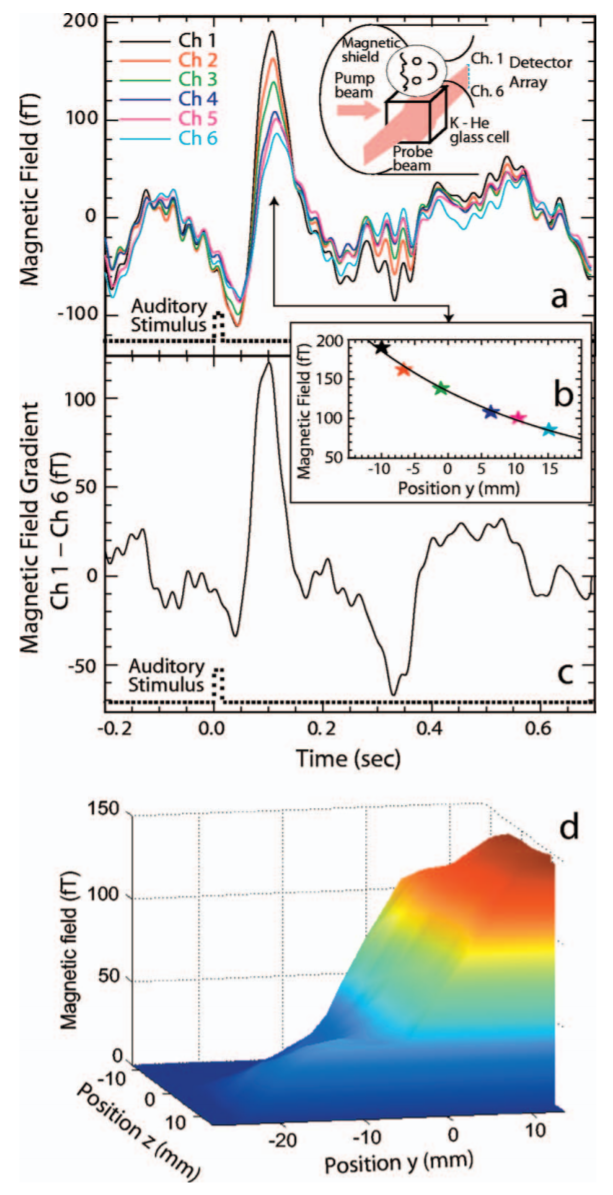
\includegraphics[height=0.7\textwidth,keepaspectratio]{MEG1}
\caption{\label{fig:MEG1} (a) Magnetic field detection averaged over 600 auditory stimuli. (b) The magnetic field gradient resulting from the difference in the position of the 6 channel photodiode which are each separated by 5mm. (c) Magnetic field gradient detection from the difference in the magnetic field signal between outer photodiode detectors in the vertical array. (d) Magnetic field detection using a 2D photodiode array \citep{XiaMagnetoencephalographyMagnetometer}.}
\end{figure}

This section discusses the schemes used and experimental results of employing a SERF AM in place of a SQUID magnetometer to complete mapping and detection of the magnetic fields produced by the human brain. In Ref. [\citen{XiaMagnetoencephalographyMagnetometer}], the first experimental MEG AM scheme was implemented. The subject lay on a bed and had their head secured above a 422 cm$^{3}$ potassium (K) vapor cell heated to 180$^{\circ}$. Between the subject and the heated vapor cell is a layer of insulating material and a water-cooling pad. The distance between the probe beam and the cooled surface is 2.5 cm. The bed is surrounded by three layers of magnetic shielding, generated by computationally controlling the magnetic fields induced by 18 coils, with an opening to fit the subjects head. 


The biomagnetic field is measured by detecting the rotation of the linearly polarised light. Prior to being detected by a 6 channel photodiode array, the linearly polarised probe light passes through polarising beam splitter orientated such that light intensity detected increases as the polarisation plane is rotated. The magnetometer is initially calibrated by applying a magnetic field which is used to measure the 3.5 fTHz$^{-1/2}$ sensitivity of the magnetometer at 10 Hz. The laser intensity fluctuations are attributed to the 1/$f$ noise spectrum. The averaged results of applying a single train of 16, 1 ms period square-wave pulses to provide an auditory stimulus is shown in Fig. (\ref{fig:MEG1}a). Therefore, the brain response to the stimuli is observed by the large peak in the magnetic field detection. The dependence on the spatial position of the photodiode detector is highlighted in Fig. (\ref{fig:MEG1}b,c). The possibility of mapping the region of the brain activated by the stimuli is illustrated in Fig. (\ref{fig:MEG1}d) where a 2D photodiode detector array is used.

\begin{figure}[b]
\centering
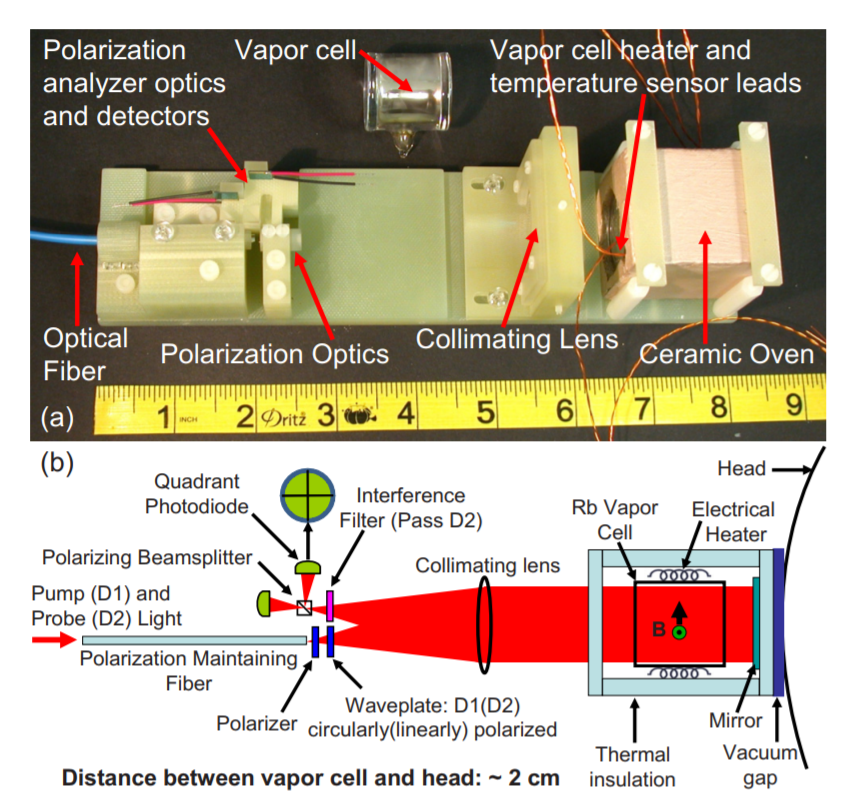
\includegraphics[height=0.4\textwidth,keepaspectratio]{MEG2a}
\caption{\label{fig:MEG2a} Atomic magnetometer (a) device photograph and (b) optical set-up. The laser field operates on a single optical axis which produces a circularly polarised D1 pump beam and linearly polarised D2 probe beam. The horizontal and vertical polarisation components of the probe are detected by separate quadrant photodiodes after the beam has been reflected back through the vapor cell \citep{Johnson2010MagnetoencephalographyMagnetometer}.}
\end{figure}

The fiber-coupled rubidium (Rb) AM shown in Fig. (\ref{fig:MEG2a}) was developed and used to complete a study of the response a subjects brain to, auditory and median nerve, stimuli which are compared to the results when using a commercial SQUID system in Ref. [\citen{Johnson2010MagnetoencephalographyMagnetometer}]. The device and has a measured sensitivity of $<$5 fTHz$^{-1/2}$ between 5-10 Hz and the subject is 2cm from the center of the cell. To increase the atomic number density to the SERF regime the cell is heated to 190 $^{\circ}$ and thermally isolated from the subject. The circularly polarised pumping enables sensitive detection of the perpendicular $B$ field where lock-in detection of the probe beam polarisation is produced using a perpendicular 1kHz modulated magnetic field. The study was completed in a shielded room where the AM required further $B$ field canceling which is achieved similarly as previously discussed for the AM design in Ref. [\citen{XiaMagnetoencephalographyMagnetometer}]. The magnetic field signal generated from the left side of the brain is detected as shown in Fig. (\ref{fig:MEG2b}).  

\begin{figure}[b]
\centering
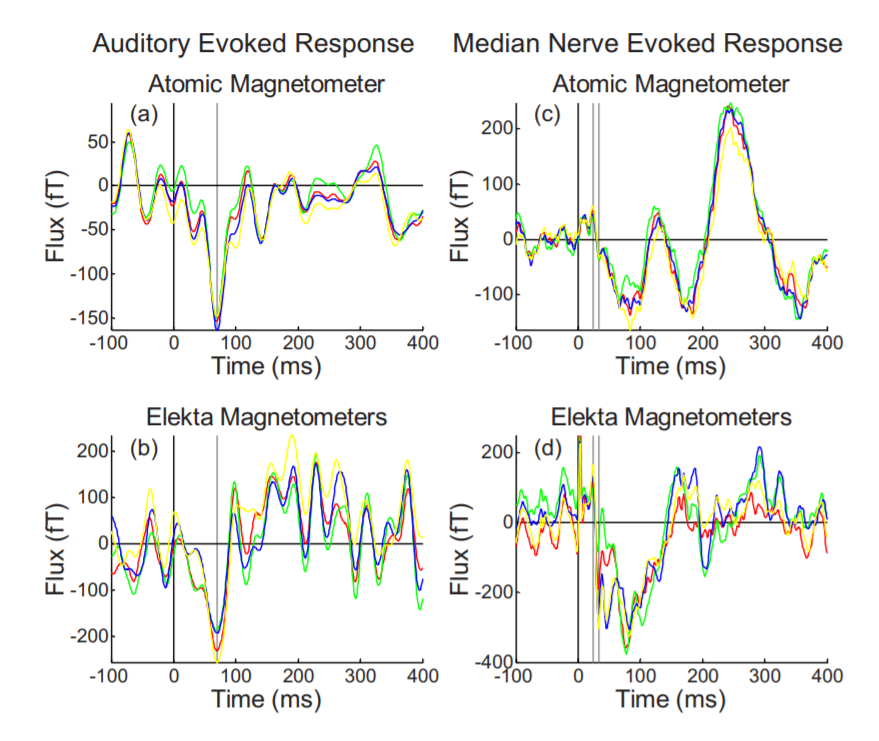
\includegraphics[height=0.43\textwidth,keepaspectratio]{MEG2b}
\caption{\label{fig:MEG2b} Magnetic flux (a) auditory and (c) right median nerve response measured by a quadrant 4-channel AM. Magnetic flux (a) auditory and (c) right median nerve response measured by four SQUIDs located near the position of the AM. The stimuli are applied at time $t=0$ s and the vertical grey lines illustrate times at which these commonly used stimuli are expected to induce responses \citep{Johnson2010MagnetoencephalographyMagnetometer}.}
\end{figure}

\begin{figure}[t]
\centering
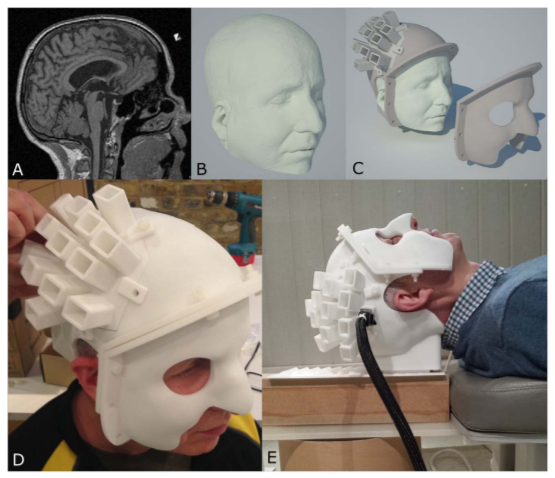
\includegraphics[height=0.4\textwidth,keepaspectratio]{MEG4a}
\caption{\label{fig:MEG4a} 3D head-cast fabrication. (a) MRI slice and (b) MRI reconstruction provided precise measure of subjects head. (c) Computer-aided design of head-cast with AM connectors for measurements of brain activity in the sensorimotor cortex. (D) The subject is wearing the 3D printed head-cast and (E) the AM attached is attached during experiment \citep{Boto2017AMagnetometers}.}
\end{figure}


The right median nerve is stimulated by a 0.8 mA electrical pulse of duration 200 $\mu$s applied to the subjects right arm and 1 kHz pulse of duration 0.25 s was used to stimulate the left audio cortex. The time between pulses is varied and the bandpass filters are used to reduce frequency noise. The magnetic field component that SQUIDs measure is perpendicular to the subject's head which is different from the component that the AM detects. Additionally the AM 4 channel detection separation is 5 mm which is smaller since the 4 SQUIDs are separated by 30 mm. Therefore, the responses which occur around 100 ms have an acceptable level of agreement and verifies that the AM has potential to provide a non-cryogenic and cheaper alternative for producing MEG systems.  

The chip-scale AM in Ref. [\citen{Sander2012MagnetoencephalographyMagnetometer.}] has a one beam optical axis but has separate optical fibers used to transmit the light to the 2 mm$^{2}$ vapor cell and from the vapor cell to the detector. The reduction in size of the device produces a reduction of the sensitivity to 200 fTH$^{-1/2}$ between 5-150 Hz. The AM measured the biomagnetic field response of the occipital region and left somatosensory cortex when the subject opens and closes their eyes and when the right median nerve is stimulated, respectively. Again the results are verified by comparison with a commercial SQUID array. AM sensitivity of $\approx$ 3 fTH$^{-1/2}$ should be attainable for this device and an increase from the 30 $\%$ efficiency of light detection will significantly improve the sensitivity. 

In Ref. [\citen{Shah2013AApplications}] an AM is presented with a similar design as in Ref. [\citen{Sander2012MagnetoencephalographyMagnetometer.}] but with a larger vapor cell and enclosed by a 50 cm$^{3}$ 3D printed casing made from plastic which can withstand the 190 $^{\circ}$ cell temperature. Magnetic coils wrapped round the thermally isolated layer remove residual magnetic fields in a magnetically shielded room. AM MEG and MCG was completed for auditory and somatosensory stimuli, respectively. The sensitivity of the AM was 10 fTHz$^{-1/2}$ when completing MEG. The significant improvement in the sensitivity of the device is attributed to the increased S/N due to the average distance between the subject and the AM surface being $<$1 cm at a frequency bandwidth of 100 Hz. 
\begin{figure}[b]
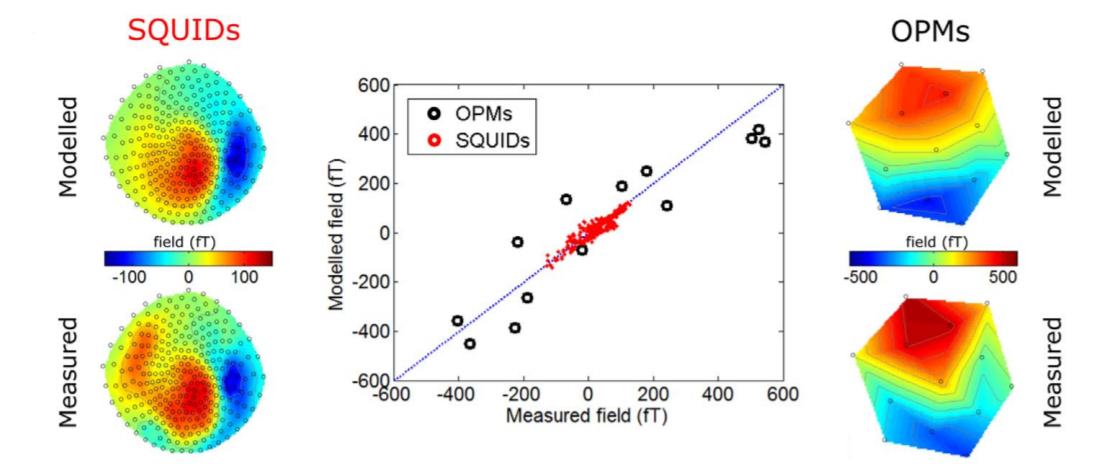
\includegraphics[height=0.23\textwidth,keepaspectratio,]{MEG5}
\caption{\label{fig:MEG5} SQUID and AM modeled and measured 2D tomographic response to the somatosensory stimuli. The center plot shows the comparison between the modeled field and the measured data \citep{Boto2017AMagnetometers}.}
\end{figure}
A similar AM device design as in Ref. [\citen{Shah2013AApplications}] was used in a study in Ref. [\citen{Boto2017AMagnetometers}] where 3D printing produced a subject specific MEG head-cast. The fabrication process is illustrated in Fig. (\ref{fig:MEG4a}). The optimum position of the 13 AMs for detection of sensory and motor response to stimuli is determined from data collected using a 275-channel commercial SQUID system. The left median nerve is stimulated using electrical pulses with a current amplitude set such that the subject's thumb twitches when the pulse is applied. Mapping of the magnetic field in response to the automotive stimuli is shown in Fig. (\ref{fig:MEG5}) for the AM and SQUID sensors. The 13-channel AM array is obtained by repeating experiment 13 times with the AM in a different position each time. The modeled tomography removes environmental interference by generating a computation gradiometer array from the measured AM and SQUID data. The computational gradiometer successfully removes the mains peak frequency in the AM detection array and the corrected sensitivity is 15.9 fTHz$^{-1/2}$ with a bandwidth > 100 Hz. The agreement between the AM modeled and measured $B$ field is very promising considering the use of only one AM to produce a 13 channel array. The AM has a dynamic range of ± 5 nT for operation in the SERF regime.
\subsection{Magnetic Induction Tomography}
Atrial fibrillation is a heart condition which is characterised by an irregular heart rate which produces abnormal conductivity of the heart tissue. Development of an noninvasive technique to diagnose and treat this condition, and possibly detect malignant tissue, using conventionality MIT has previously been unsuccessful \citep{Marmugi2016OpticalHeart}. In the conventional MIT scheme a magnetic field is generated from current flowing through the primary coil. The magnetic field induces an Eddy current in the sample material and a secondary coil is used sense the conductivity. However, the conductivity of the biological material is very small which limits the ability detect the magnetic field induced \citep{Griffiths2001MagneticTomography}. 






A noval MIT scheme has been developed in Ref.[\citen{Deans2016ElectromagneticMagnetometer}] which uses an all optical pump-probe AM and applies an rf magnetic field to drive atoms from the Dark states. The result is rf polarisation rotation of the probe beam. Therefore changes in the phase or amplitude of the detected probe light due to Eddy currents in the biological tissue enables mapping of tissue conductivity. In Ref. [\citen{Deans2016OpticalHeart}] the dynamic range of the sensing device is illustrated by completing MIT of metal samples where the known conductivity of one sample is two orders of magnitude larger than the other. The future implication for diagnosing heart conditions, of accurate MIT regardless of the sample conductivity, is highlighted in Fig. (\ref{fig:MIT}).

\begin{figure}[h]
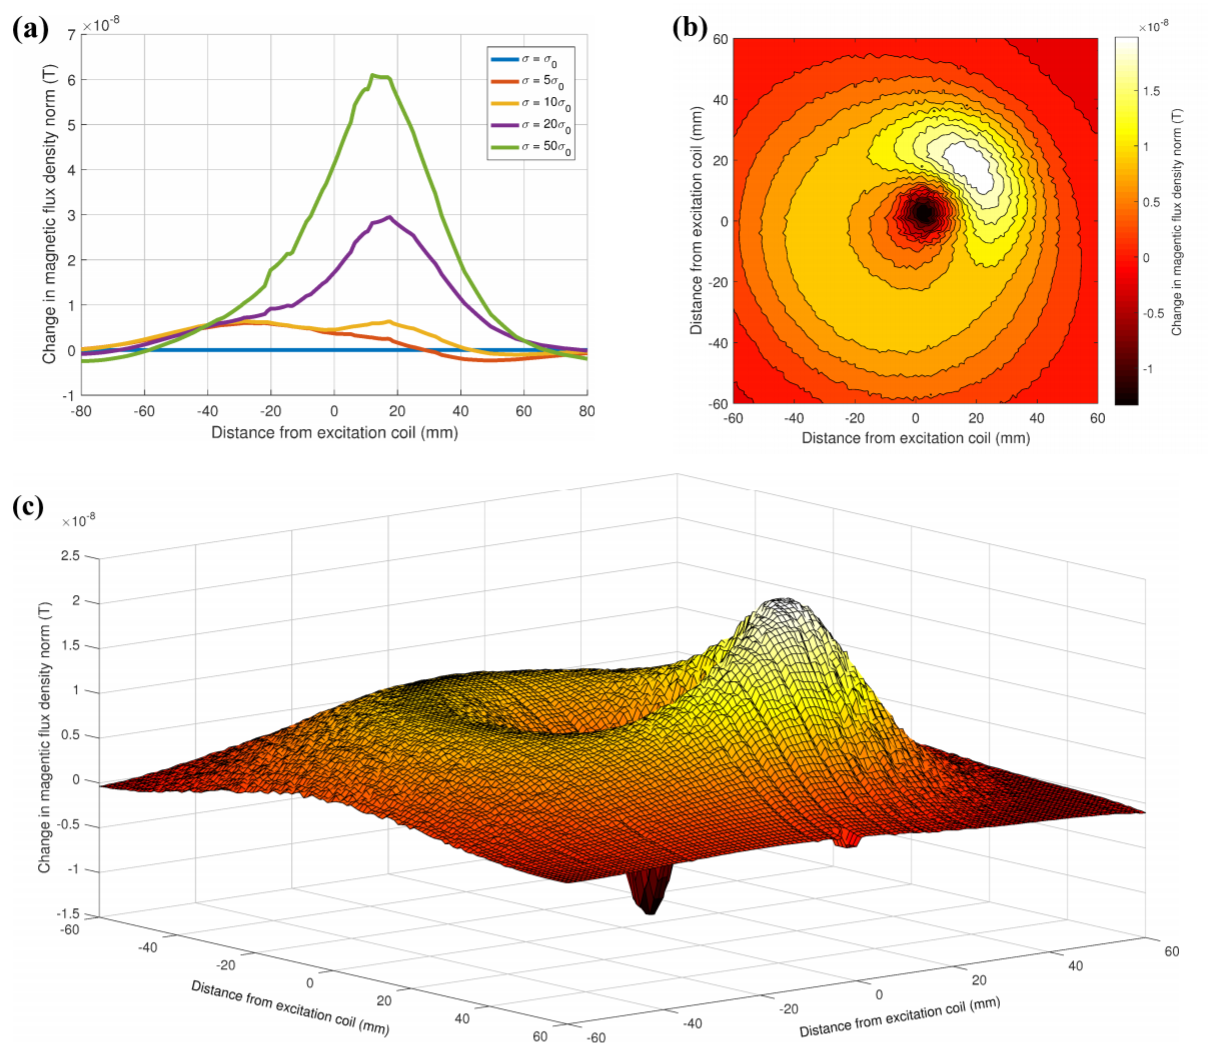
\includegraphics[height=0.42\textwidth,keepaspectratio,]{MIT}
\caption{\label{fig:MIT}(a) Change in the magnetic flux due to due variation in anomaly conductivity, where $\sigma_{0}=0.875 Sm^{1}$. Heart anomaly contour plot in (b) 2D and (c) 3D \citep{Deans2016OpticalHeart}.}
\end{figure}


\par

\section{Outlook}

The experimental research completed to investigate the suitability of AMs as a lower-costing alternative for multi-channel detection of biomagnetic fields of the human brain are discussed in Sec. \ref{sec:level1}. The results provide preliminary promising results where the AM response to sensory, auditory, spontaneous and motive stimuli are deemed to be within an acceptable agreement with the commerical SQUID detection system. Additionally, in Ref. [\citen{XiaMagnetoencephalographyMagnetometer}] the human sized magnetic shielding developed illustrates the improvement of using AMs compared to SQUIDs. The measured sensitivity of the AM in Ref. [\citen{Shah2013AApplications}] is comparable to the operation of commercial SQUID devices. However, due to the limited bandwidth the AM operation they may not be suitable of measurement of all applications of MEG. 

The progress made in Ref. [\citen{Boto2017AMagnetometers}] constructing a 3D printed head-cast to host the AM sensing devices further illustrates benefits of operation at non-cryogenic temperatures. Therefore the AMs can be attached to the head-cast such that there is a 6.5 mm distance between the center of the sensing area and the patients skin. The benefit is an increased S/N and detection of deeper magnetic fields. Additionally, further advantages include the possibility of providing patient specific head-casts, similarly to providing patient head-molds for radiotherapy treatment, and the flexibility in AM positioning. The next stage would be to fabricate more AMs and complete multiple-channel detection to investigate correlations with the 13 channel detection completed using one AM. The rf AM used for MIT shows promising initial results for future implementation to detect and diagnose abnormalities in biological tissue detected from atypical tissue conductivity.   
  
  





\bibliographystyle{ieeetr}

\bibliography{main}

\end{document}